\section{Gate-level results}
\subsection{Gates, corners and SPICE reference}
The five gates INV, NAND2, NOR2, AND2 (NAND2 followed by INV) and OR2 (NOR2 followed by INV) are static CMOS circuits; AND2 and OR2 are simulated in SPICE as complete gates.
The transistor widths are (in multiples of $L_{\min}$): INV $W_n=1,W_p=2$; NAND2 $W_n=2,W_p=2$; NOR2 $W_n=1,W_p=4$ (assumption, Appendix~\ref{app:assumptions}).
A corner is one random draw of $V_{DD}$, temperature and process parameters; all NMOS of a gate share one process draw and all PMOS another. The same 200 corners are used for every gate,
every input combination, and later for the test circuit, giving $18\times200=3600$ SPICE runs. Gate inputs are exactly $0$ or $V_{DD}$. A 0\,V source in the ground rail
makes the return current measurable, so that Kirchhoff's law can be verified on every run: all source currents sum to zero within $10^{-3}$ of the largest one (checked by the test-suite
for every gate case).

\paragraph{Gate leakage definition.} The leakage is the total current delivered by all sources at $V_{DD}$ (supply plus inputs held high), which equals the current absorbed by the sources at $0$\,V.

\paragraph{Validity of the SPICE reference.} With exactly the mandated solver options, ngspice returned an invalid operating point in 59 of the 3600 runs (e.g.\ the inverter output of an
AND2 stuck at $7\times10^{-5}$\,V instead of $4\times10^{-8}$\,V, giving a leakage 200 times too large, in one case even negative) and did not converge at all in 66 more runs. All runs
were therefore solved twice: with exactly the mandated options, and with one additional options line that sets abstol to the numerical noise floor ($10^{-15}$\,A) and tightens reltol/vntol.
The mandated result is the reference whenever it agrees with the tight solve within 1\,\%; otherwise the tight solve is used (Table~\ref{tab:ref}). The mandated \texttt{.options} line stays in every netlist.
\begin{table}[H]
\centering
{\small
\begin{tabular}{lrl}
\toprule
reference source & runs & meaning \\
\midrule
mandated & 3475 & mandated-option solve (agrees with tight cross-check within 1\%) \\
tight\_only & 66 & mandated solve did not converge -> tight solve used \\
tight & 59 & mandated solve disagreed with the cross-check -> tight solve used \\
\bottomrule
\end{tabular}
}
\caption{Origin of the 3600 gate SPICE reference values.}
\label{tab:ref}
\end{table}



\subsection{From transistor currents to gate leakage}\label{sec:gates_method}
For each run the SPICE-recorded node voltages (internal node, NAND/NOR output, gate output) give the terminal voltages $(V_d,V_g,V_s,V_b)$ of every transistor; each transistor is routed to the ON model of its
type if its gate voltage is on the conducting side of $V_{DD}/2$, else to the OFF model; the four predicted currents follow from the chosen model.

A plain sum of the predicted terminal currents at the nodes held at $V_{DD}$ (or, alternatively, at $0$\,V) turned out to be unusable (Table~\ref{tab:estimators}): in a leaking gate the ON
transistors carry only the leakage current of the blocking network, at a drain-source voltage of about $10^{-7}$\,V, a regime in which the channel current is $g\,V_{ds}$ with $g\approx10^{-4}$\,S. The ON model, accurate to a few percent
of the ON-state currents, cannot resolve a $3\times10^{-11}$\,A current there; the sums are dominated by its absolute error (median error $\approx100\%$, even negative leakage).
The channel current of an ON transistor is not something to predict but is fixed by Kirchhoff's current law, so the following KCL-consistent composition is used:
for every ON transistor the channel current $J$ is an unknown, its other channel terminal follows from device conservation ($I_s=-J-I_g-I_b$), the gate and body currents are taken from the ML model, and
the node equations of the internal nodes of the gate are solved for the $J$ in the least-squares sense. The leakage is then summed at the rails; the result of the supply side and of the ground side agree closely
(Table~\ref{tab:estimators}) and their mean is reported. Only the OFF-state predictions and the gate/body currents --- the quantities the models predict well --- determine the result.
\begin{table}[H]
\centering
{\small
\begin{tabular}{lrrrr}
\toprule
estimator & bias & median err & 95th pct err & mean err \\
\midrule
plain sum of terminal currents at the VDD-level nodes & -186.2 & 0.9984 & 1460 & 292.7 \\
plain sum of terminal currents at the 0 V-level nodes & 533.3 & 1.954 & 1761 & 539.1 \\
KCL-consistent, supply side & 0.01505 & 0.05557 & 0.1964 & 0.07242 \\
KCL-consistent, ground side & 0.01512 & 0.05511 & 0.1947 & 0.07222 \\
KCL-consistent, mean of both (reported) & 0.01508 & 0.05529 & 0.1956 & 0.07214 \\
\bottomrule
\end{tabular}
}
\caption{Gate-level error of the alternative ways of turning predicted transistor currents into gate leakage (all 3600 runs; fractions, not percent).}
\label{tab:estimators}
\end{table}



\subsection{Results}
\begin{table}[H]
\centering
{\small
\begin{tabular}{lrrrrr}
\toprule
case & SPICE median [A] & ML median [A] & bias & median err & 95th pct err \\
\midrule
INV\_0 & $3.29\times10^{-11}$ & $3.15\times10^{-11}$ & 1.05\% & 5.30\% & 17.54\% \\
INV\_1 & $2.60\times10^{-11}$ & $2.62\times10^{-11}$ & 1.51\% & 7.78\% & 23.79\% \\
NAND2\_00 & $5.69\times10^{-11}$ & $5.91\times10^{-11}$ & 2.25\% & 5.18\% & 16.88\% \\
NAND2\_01 & $1.19\times10^{-10}$ & $1.15\times10^{-10}$ & 1.15\% & 5.88\% & 17.94\% \\
NAND2\_10 & $3.30\times10^{-11}$ & $3.31\times10^{-11}$ & 2.68\% & 5.05\% & 15.46\% \\
NAND2\_11 & $1.24\times10^{-10}$ & $1.15\times10^{-10}$ & -0.60\% & 8.37\% & 27.74\% \\
NOR2\_00 & $1.31\times10^{-10}$ & $1.34\times10^{-10}$ & 2.34\% & 5.31\% & 17.74\% \\
NOR2\_01 & $1.11\times10^{-10}$ & $1.14\times10^{-10}$ & 1.67\% & 4.95\% & 15.44\% \\
NOR2\_10 & $2.53\times10^{-11}$ & $2.46\times10^{-11}$ & 1.70\% & 7.76\% & 24.35\% \\
NOR2\_11 & $3.95\times10^{-11}$ & $3.85\times10^{-11}$ & 2.14\% & 8.28\% & 24.75\% \\
AND2\_00 & $9.60\times10^{-11}$ & $9.58\times10^{-11}$ & 1.92\% & 4.11\% & 14.45\% \\
AND2\_01 & $1.42\times10^{-10}$ & $1.36\times10^{-10}$ & 0.99\% & 5.17\% & 17.05\% \\
AND2\_10 & $6.90\times10^{-11}$ & $7.19\times10^{-11}$ & 1.79\% & 4.15\% & 16.39\% \\
AND2\_11 & $1.77\times10^{-10}$ & $1.78\times10^{-10}$ & 0.50\% & 6.52\% & 19.89\% \\
OR2\_00 & $1.83\times10^{-10}$ & $1.78\times10^{-10}$ & 2.29\% & 4.71\% & 15.91\% \\
OR2\_01 & $1.45\times10^{-10}$ & $1.45\times10^{-10}$ & 1.51\% & 4.39\% & 14.93\% \\
OR2\_10 & $6.81\times10^{-11}$ & $7.01\times10^{-11}$ & 1.17\% & 4.53\% & 16.48\% \\
OR2\_11 & $9.29\times10^{-11}$ & $9.06\times10^{-11}$ & 1.09\% & 5.54\% & 17.41\% \\
\bottomrule
\end{tabular}
}
\caption{Gate-level results for the 18 gate/input cases (200 corners each). Error is $|I_{ML}-I_{SPICE}|/I_{SPICE}$; bias is the mean signed relative error.}
\label{tab:gates}
\end{table}


\begin{table}[H]
\centering
{\small
\begin{tabular}{lrrrrr}
\toprule
gate & runs & bias & median err & 95th pct err & mean accuracy \\
\midrule
INV & 400 & 1.28\% & 6.20\% & 22.04\% & 91.76\% \\
NAND2 & 800 & 1.37\% & 5.83\% & 20.93\% & 92.33\% \\
NOR2 & 800 & 1.96\% & 6.31\% & 22.54\% & 91.76\% \\
AND2 & 800 & 1.30\% & 4.95\% & 17.38\% & 93.52\% \\
OR2 & 800 & 1.52\% & 4.75\% & 16.12\% & 94.05\% \\
\bottomrule
\end{tabular}
}
\caption{Gate-level accuracy per gate type.}
\label{tab:bygate}
\end{table}


\begin{figure}[H]\centering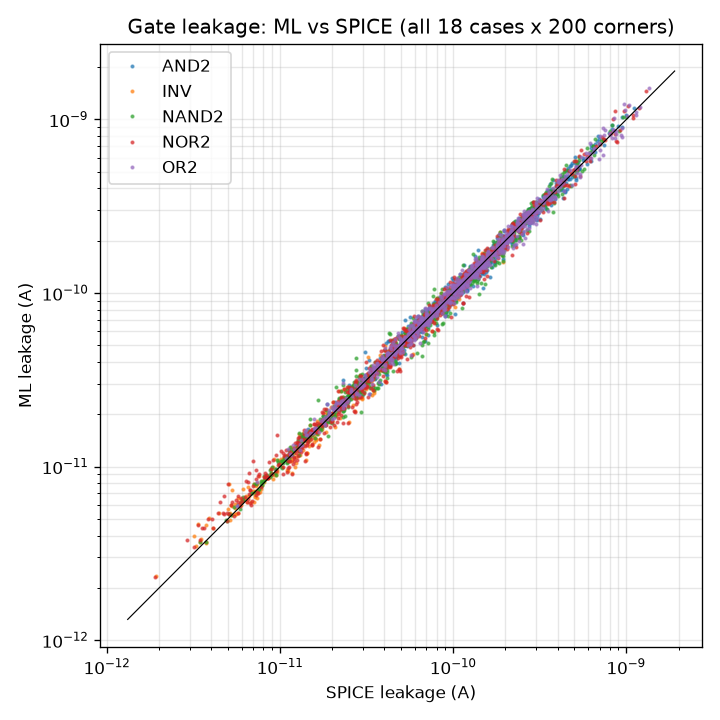
\includegraphics[width=.72\textwidth]{gate_parity.png}\caption{ML versus SPICE leakage for all 3600 gate simulations (log axes).}\label{fig:gparity}\end{figure}
Over all 3600 runs the median error is 5.5\,\%, the 95th percentile 19.6\,\%, the largest error 59\,\%, the bias $+1.5$\,\% and the mean accuracy ($1-$ mean relative error) 92.8\,\%.
The gates ending in an inverter (AND2, OR2) are the most accurate (median 4--6\,\%), probably because their leakage is the sum of two stages whose errors partly average out (not isolated by a separate experiment). The least accurate cases are
INV with input 1, NAND2 with inputs 11, and NOR2 with inputs 10 and 11 (median about 8\,\%): in all of them the leakage flows through OFF \emph{PMOS} transistors, and the PMOS OFF model is the least accurate of the four
(Section~\ref{sec:models}). Cases whose leakage is set by OFF NMOS transistors (e.g.\ NAND2 with inputs 00, 01, 10) reach median errors near 5\,\%.
